\documentclass{standalone}
\usepackage{pgfplots}
\pgfplotsset{compat=1.18}
\usepackage{subcaption}

\begin{document}

\begin{figure}
\centering
\begin{subfigure}{0.48\textwidth}
    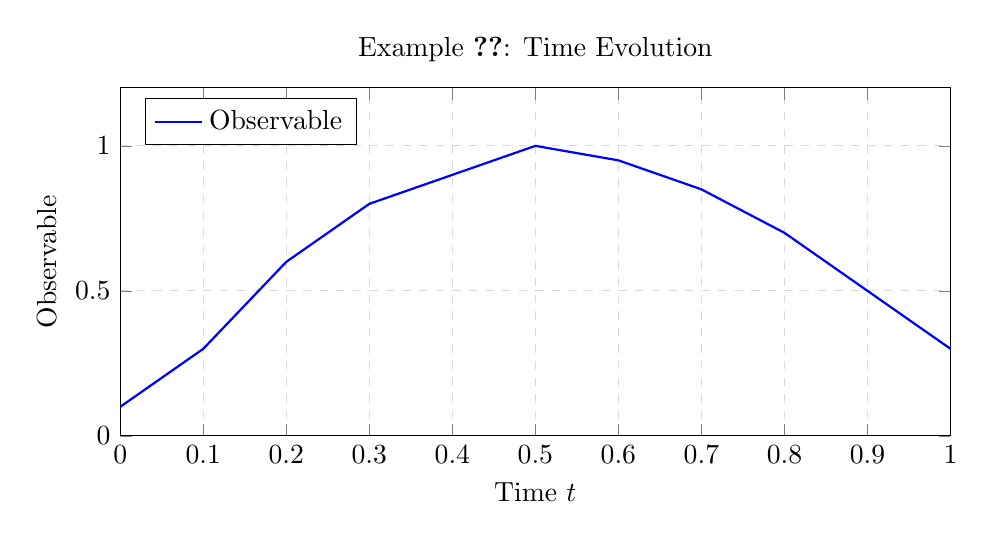
\begin{tikzpicture}
    \begin{axis}[
        width=\linewidth,
        height=6cm,
        xlabel={Time $t$},
        ylabel={Observable},
        grid=both,
        grid style={dashed, gray!30},
        title={Example \ref{ex: matrix, nonlinear, time-independent}: Time Evolution},
        xmin=0, xmax=1,
        ymin=0, ymax=1.2,
        legend pos=north west,
    ]
    % Sample data (replace with actual data)
    \addplot[blue, thick] coordinates {
        (0, 0.1) (0.1, 0.3) (0.2, 0.6) (0.3, 0.8)
        (0.4, 0.9) (0.5, 1.0) (0.6, 0.95)
        (0.7, 0.85) (0.8, 0.7) (0.9, 0.5) (1, 0.3)
    };
    \legend{Observable}
    \end{axis}
    \end{tikzpicture}
\end{subfigure}
\hfill
\begin{subfigure}{0.48\textwidth}
    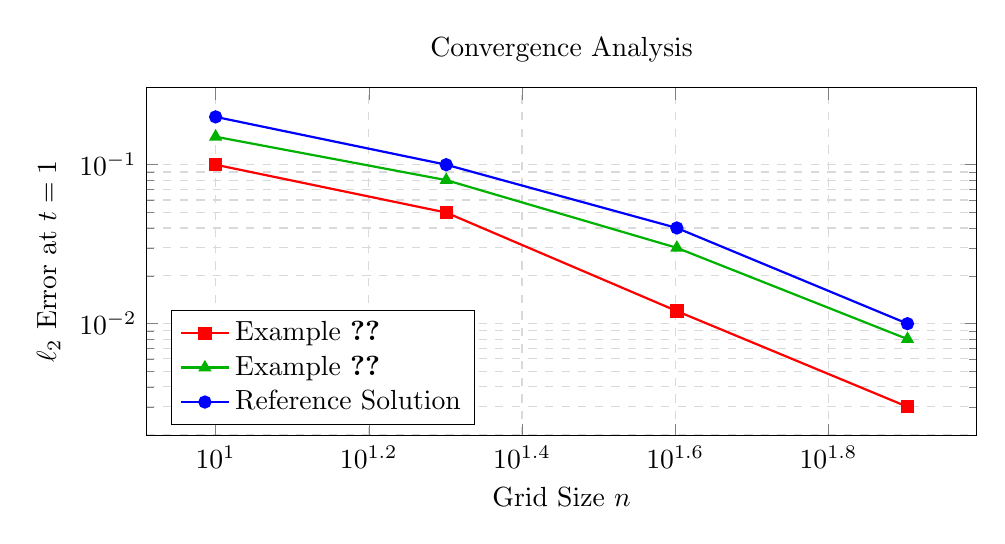
\begin{tikzpicture}
    \begin{axis}[
        width=\linewidth,
        height=6cm,
        xlabel={Grid Size $n$},
        ylabel={$\ell_2$ Error at $t=1$},
        grid=both,
        grid style={dashed, gray!30},
        title={Convergence Analysis},
        xmode=log,
        ymode=log,
        legend pos=south west,
        legend cell align={left}
    ]
    % Sample convergence data (replace with actual data)
    \addplot[red, mark=square*, thick] coordinates {
        (10, 0.1) (20, 0.05) (40, 0.012) (80, 0.003)
    };
    \addplot[green!70!black, mark=triangle*, thick] coordinates {
        (10, 0.15) (20, 0.08) (40, 0.03) (80, 0.008)
    };
    \addplot[blue, mark=*, thick] coordinates {
        (10, 0.2) (20, 0.1) (40, 0.04) (80, 0.01)
    };
    \legend{
        Example \ref{ex: matrix, nonlinear, time-dependent},
        Example \ref{ex: matrix, nonlinear, time-independent},
        Reference Solution
    }
    \end{axis}
    \end{tikzpicture}
\end{subfigure}
\caption{Left: Temporal evolution of system observables. Right: Numerical convergence comparison for nonlinear matrix examples.}
\end{figure}

\end{document}